\documentclass[pdftex,12pt,a4paper]{report} 

% Document settings

\usepackage{fullpage}
\usepackage{cite}
\usepackage{datetime} 
\usepackage{geometry}
\usepackage[pdftex]{graphicx}
\usepackage{verbatim}
\usepackage{todonotes}
\usepackage{array}
\usepackage[pdftex]{graphicx}
\usepackage{capt-of}
\usepackage[parfill]{parskip}

\geometry{verbose,lmargin=3cm,rmargin=3cm}

\newcommand{\HRule}{\rule{\linewidth}{0.5mm}}

\begin{document}

\title{Computer Music Improvisation - Grammatical Approach For Blues}
\author{Cliff Sun (chs09)}
\date{November 2012}
\maketitle

\begin{abstract}

Write the abstract last.



Improvisation is a very interesting topic in the world of music. There are many factors that influence how a musician improvises with an instrument. In addition blues has simple rules and allows the player to take any sort of musical direction they want. Here we will be looking at a grammatical and symbolic approach to generating blues music on top of a  simple twelve bar blues accompaniment. 

\end{abstract}

\setcounter{tocdepth}{2} % Set the depth of toc indexing

\tableofcontents

\pagebreak

\renewcommand*\thesection{\arabic{section}}

% \section{Acknowledgements}

% acknowledge

\pagebreak

\chapter{Introduction}

\section{Project Introduction}
Improvisation is often seen as a human activity, especially in the domain of music. Genre's such as Jazz and Blues are heavily based on the performer improvising on a set form. Improvisation itself is essentially just a set of skills and techniques that need to be mastered just like any other activity so it is not to say that a computer can't 'improvise'. The aim of this project is to be able to model and replicate such music improvisation using a computer. The area of computational creativity in music has been explored before and is still ongoing, and we hope that this project can provide a new approach for computer music improvisation.

\paragraph{Improvisation vs Composition}
Music improvisation can be defined as the creative activity of immediate composition, or 'Composition on the fly'. In the case of our project when we talk about composition, it means the same thing as improvisation.


\section{Blues Improvisation}
Blues is one of the most common genres that relies on performer improvisation. Performers of this genre tend to play a musical instrument (including voice) on top of an accompaniment with a well defined structure/form. The blues form itself is often defined by its 12 bar chord progression (commonly called 12 bar blues) which is essentially a standard harmonic chord progression of 12 bars in a standard 4/4 time signature. Table 1.1 below shows the chords for the general 12 bar blues form, with I7 referring to the harmonic seventh Tonic chord. Chord IV refers to the 'dominant' chord (4th degree) and Chord V refers to the 'dominant' chord (4th degree).


\begin{table}[here]
\centering
\newcolumntype{C}{>{\centering\arraybackslash}m{23pt}<{}}
\begin{tabular}{|*{12}{C|}}
  I & I or IV & I & I7 & IV & IV & I & I7 & V & V or IV & I & I or V
\end{tabular}
\caption{12 bar blues chord progressions}
\label{12 bar blues}
\end{table}


\begin{table}[here]
\centering
\newcolumntype{C}{>{\centering\arraybackslash}m{23pt}<{}}
\begin{tabular}{|*{12}{C|}}
  I & I & I & I & IV & IV & I & I & V & IV & I & I
\end{tabular}
\caption{12 bar blues simplified chord progression}
\label{12 bar blues}
\end{table}


Table 1.2 gives us one possible (and simple) chord progression for 12 bar blues in which we will basing our improvisation upon. 


\subsection{Blue Notes} What really gives the blues genre it's characteristics are the 'blue notes'. These are notes which are played at a lower pitch (flatter) than that of the major scale (usually one semitone lower on piano). The notes which are 'flattened' are the \textbf{third}, \textbf{fifth} and \textbf{seventh} notes of the major scale.
There are theoretical reasons for the introduction of 'blue notes' which we won't go into detail here. But essentially these 'blue notes' allow for moments of expression in blues melodies. 

\subsection{Blues and Pentatonic Scales}
Blues scales include the blue notes that we've mentioned above, these scales give the performer a set of notes to improvise with and gives the music the characteristic 'blues' feel to it. Blues scales are generally based on the major/minor pentatonic scale. A pentatonic scale is a scale of five notes (compared to seven notes in regular major/minor scale) and is widely used in music across the world. The most common blues scale (and the one we are going to be basing our improvisations on) is the blues minor scale which is based on the minor pentatonic scale (see Figure \ref{fig:cminorpentatonicscale}) with a sharp 4th note (or a flat 5th note, both are equivalent). In Figure \ref{fig:cminorbluesscale} we can see the blues minor scale includes all the blue notes; E(3rd degree) flat, G(5th degree) flat and B(7th degree) flat.


\begin{figure}[here]
  \centering
  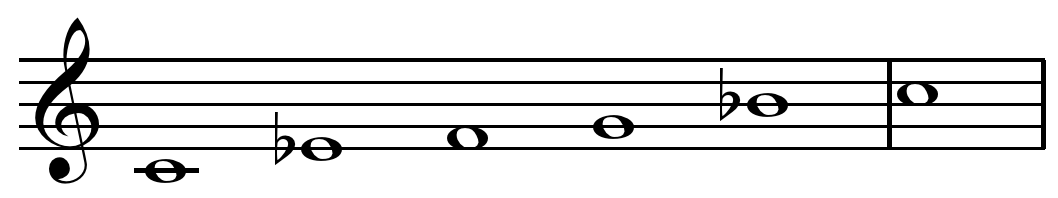
\includegraphics[scale=0.3]{figure/minorpentatonicscale.png}
  \captionof{figure}{C minor pentatonic scale}
  \label{fig:cminorpentatonicscale}
\end{figure}

\begin{figure}[here]
  \centering
  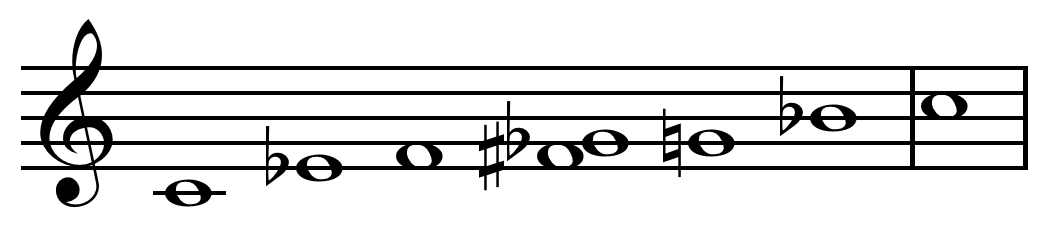
\includegraphics[scale=0.3]{figure/bluesminorhexatonicscale.png}
  \captionof{figure}{C minor blues (hexatonic) scale}
  \label{fig:cminorbluesscale}
\end{figure}


\section{Computer Improvisation For Blues}
Using the characteristics of blues music, we can limit our musical domain which simplifies the overall problem. Our aim is to be able to generate/improvise blues melodies on top of a standard 12 bar blues progression using a computer. The above explanations on blues scales and chord progression only concerns the pitch characteristics of blues music. The issue of rhythm and structure is just as crucial in defining blues music and has yet to be discussed. There are many different approaches to such a problem and many of them have involved a statistical/machine learning approach. We propose a more grammatical approach to composing and generating blues melodies which will allow us to create well-defined structures and rhythms for blues melodies. The next chapter explains this in detail. In addition we hope to include a genetic/evolutionary part to the improvisation which will allow the computer to improvise in a more human-like way, i.e. variation and invention of new melodies/licks using previous/current knowledge.

\paragraph{Keys}
For simplicity, everything we do (melody generations/chord progressions) will be done in the key of C. We will be basing improvisations on the C minor blues scale and use a simplified 12 bar blues progression in the key of C.

\pagebreak

\chapter{Grammar For Blues}

\section{Introduction}
In this project we propose a grammatical approach for generating blues melodies.  Grammars enforce structures within music and such a linguistic approach seems suitable for the 'call and response' nature of African-American influenced music such as blues. We can compare a line of melody to a sentence in natural language. For example a sequence of notes and the rhythm that they occur in gives a melody it's own character and meaning, like a sentence in natural language. However in music there are no semantic rules in terms of the melody, it is entirely up to the listener/player as to how they interpret it. This is where a grammar comes in, grammars are structural rules that govern the composition of 'sentences' (in the case of natural language) and such grammars are not concerned with the semantics of the sentence. Therefore a well-defined grammar for blues music should be able to produce well-structured blues melodies.


\subsection{Natural Language Grammars (Don't add this to final version)}
In the english language grammar, the language constructs consist of Nouns, Verbs, Adjectives, Determiners, Prepositions, Adverbs etc. For example if we have a sentence such as \textit{The black cat sat on the brown mat}, then we can analyse the grammatical structure of such a sentence.


\section{Initial Non-Grammatical Approach}

Before diving into a grammatical approach for blues melody improvisations, we decided to explore some simple ideas regarding probabilistic generation of notes in a sequence. Below are two simple approaches that we took. Note that we could easily classify these approaches with a simple grammar, however the point of introducing a grammar is so that we can defined structure and rhythm in our melodies, so for now we say that the first two simple approaches/implementations are not a 'grammatical' approach.

\subsection{Probablistic Randomisation (with fixed duration)}
We decided to make a quick music improvisation tool which uses probabilities to pick the next note in the melody. We kept the duration constant (a quaver/eighth note) and kept the range within one octave. An example of the generation is shown below in Figure \ref{fig:randomgeneration}. We designed it so that the probability that we choose the next note has an inverse relation to the interval of the note itself. I.e. the probability is of choosing an adjacent note in the blues scale is highest, with the probability for choosing a note that is 2 notes apart lower. In addition we made it so that the probability that we choose a note so that sequence is going in the same direction is higher than choosing a note that changes the direction of the sequence. For example if we had an F (natural) followed by an F\#, the probability of choosing G is higher than choosing an F (natural) (both one note interval from F\#).

\begin{figure}[here]
  \centering
  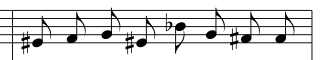
\includegraphics[scale=0.7]{figure/randomgeneration.png}
  \captionof{figure}{Probabilistic Generation for A Blues Sequence}
  \label{fig:randomgeneration}
\end{figure}

In the figure above we can see that a probabilistic random generation of notes with some constraints yields a fairly decent result. The notes are all part of the blues scale and so sound acceptable as a blues melody, however it lacks structure and rhythm as all the notes are of the same duration. 

\subsection{Probabilistic Randomisation With Mixed Durations}

To add some rhythm to the melody we decided that we could randomly choose duration lengths when we chose the next note. In our implementation we limited ourselves to semiquaver (16th), quaver (8th), and crotchet (quarter) notes. The idea was to introduce some style of rhythm to the music in the hopes of trying to make the melody fit into the blues criteria.

In Figure \ref{fig:randomgenerationwithdifferentdurations} we can see that choosing a random duration can give decent results. In our case we have an example of syncopation with the Eb quaver being played half a beat after the second beat. This sounds interesting and much more like blues music than in the previous example (in section 3.1). However not all bars generated look like this, some don't sound pleasing at all and some sound wrong rhythmically. As we are generating random durations, we are generating random rhythms and sequences and we may occasionally get a good melody, but a lot of the time we get bad or awkward rhythms. 

\begin{figure}[here]
  \centering
  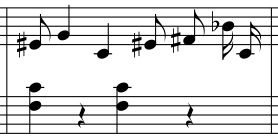
\includegraphics[scale=0.6]{figure/randomgenerationdifferentdurations.png}
  \captionof{figure}{Probabilistic Generation for A Blues Sequence}
  \label{fig:randomgenerationwithdifferentdurations}
\end{figure}


\section{Adding a Grammar For Blues}
The initial approaches are promising and give us a good foundation to build upon. If we randomly choose notes from a blues scale, they generally sound acceptable/good in terms of the pitch. However we have identified that some of the melodies/bars do not sound good rhythmically, i.e. they either don't sound good at all, or don't have the blues characteristics. We can see now that the rhythm of the notes is just as important as the pitch of the notes. The idea of creating a grammar for blues means that we can control aspects of the rhythm whilst allowing the pitch of the notes to be controlled in another way. This way we hope to be able to generate full melodies that satisfies the blues characteristics and more importantly sound pleasing to the listener.

In addition, musical melodies are generally based on a recurring theme, i.e. a small pattern which is then embellished by different variations, thus giving the listener a sense of identity for the song. The introduction of a grammar may also be able to enforce this.

\subsection{Context-Free Grammars}
A Context-Free grammar is a grammar 
The majority of natural languages can be said to be based on context-free grammars

\end{document}


